\documentclass[12pt,a4paper]{article}

% Packages
\usepackage{geometry}
\usepackage{graphicx}
\usepackage{titling}
\usepackage{hyperref}
\usepackage{longtable}
\usepackage{booktabs}
\usepackage{xcolor}
\usepackage{caption}
\usepackage{enumitem}
\usepackage{amsmath}
\usepackage{tikz}
\usepackage{listings}
\usepackage{datetime}
\usepackage{microtype}
\usetikzlibrary{shapes.geometric, arrows, positioning, fit, calc}

% Page Setup
\geometry{top=2.5cm, bottom=2.5cm, left=2.5cm, right=2.5cm}
\hypersetup{
    colorlinks=true,
    linkcolor=blue,
    filecolor=magenta,      
    urlcolor=cyan,
    pdftitle={CNSMS Project Report},
}

% Code Listings Style
\definecolor{codegreen}{rgb}{0,0.6,0}
\definecolor{codegray}{rgb}{0.5,0.5,0.5}
\definecolor{codepurple}{rgb}{0.58,0,0.82}
\definecolor{backcolour}{rgb}{0.95,0.95,0.92}

\lstdefinestyle{mystyle}{
    backgroundcolor=\color{backcolour},   
    commentstyle=\color{codegreen},
    keywordstyle=\color{magenta},
    numberstyle=\tiny\color{codegray},
    stringstyle=\color{codepurple},
    basicstyle=\ttfamily\small,
    breakatwhitespace=false,         
    breaklines=true,                 
    captionpos=b,                    
    keepspaces=true,                 
    numbers=left,                    
    numbersep=5pt,                  
    showspaces=false,                
    showstringspaces=false,
    showtabs=false,                  
    tabsize=2
}
\lstset{style=mystyle}

% Metadata
\title{\textbf{Campus Navigation and Safety Management System (CNSMS)}}
\author{
    Muhammad Hanzala (232201020) \\
    Haseeb Nawaz (232201011) \\
    Third Member (232201015) \\[1em]
    \textit{Supervisor: Sir Uzair Hassan} \\
    \textit{Subject: Web Technology}
}
\date{\today}

\begin{document}

\maketitle
\begin{abstract}
    This report documents the design and implementation of the Campus Navigation and Safety Management System (CNSMS), a web-based platform designed to enhance campus security. The system integrates a Python Flask backend with an Android mobile client, enabling real-time incident reporting, AI-based severity analysis, and interactive safety mapping. Key features include a hybrid authentication system supporting both web sessions and JWT tokens, a role-based access control model, and a scalable database schema. This document helps technical stakeholders understand the system architecture, API specifications, and deployment procedures.
\end{abstract}

\tableofcontents
\newpage

\section{Introduction}
\subsection{Motivation}
Traditional campus security reliance on manual phone reporting or physical patrols often leads to delayed response times and a lack of centralized data. The CNSMS project aims to digitize this process, providing students with an immediate reporting tool and security officers with a real-time command dashboard.

\subsection{Scope & Objectives}
The project scope includes:
\begin{itemize}
    \item \textbf{Mobile Reporting}: Allowing students to capture images and location data of incidents.
    \item \textbf{Central Dashboard}: Providing admins with a visual map of active threats.
    \item \textbf{AI Analysis}: Automating the prioritization of incidents (e.g., detecting fire vs. litter).
\end{itemize}
\textbf{Out of Scope}: Real-time video streaming, hardware sensor integration.

\section{System Overview}
The system follows a client-server architecture with a clear separation between the frontend (Android/Web Stats) and the backend (Flask API).

\begin{figure}[h]
    \centering
    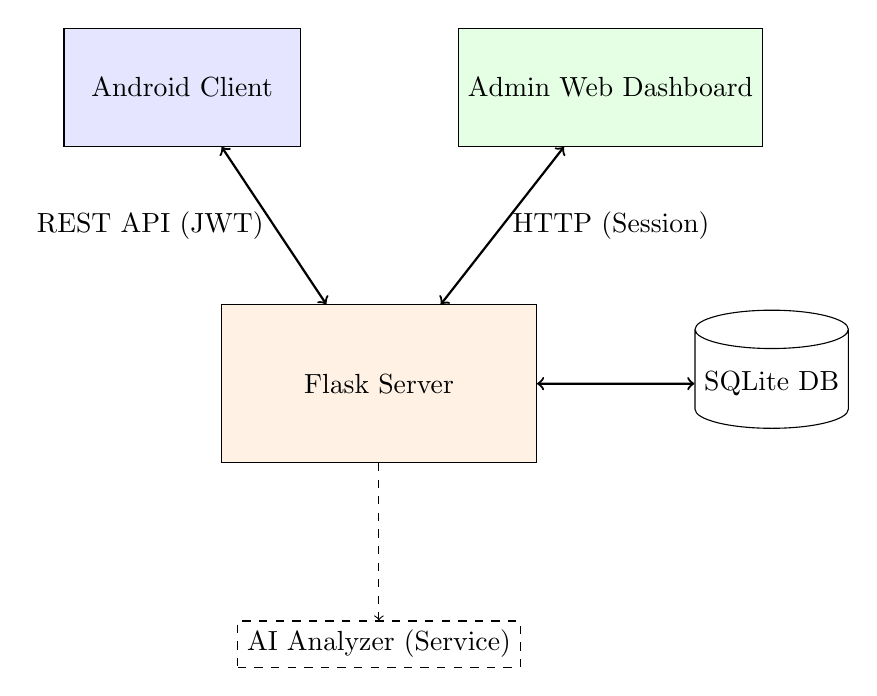
\begin{tikzpicture}[node distance=2cm]
        \node (android) [rectangle, draw, minimum width=3cm, minimum height=1.5cm, fill=blue!10] {Android Client};
        \node (web) [rectangle, draw, minimum width=3cm, minimum height=1.5cm, fill=green!10, right=of android] {Admin Web Dashboard};
        
        \node (server) [rectangle, draw, minimum width=4cm, minimum height=2cm, fill=orange!10, below=of android, xshift=2.5cm] {Flask Server};
        
        \node (db) [cylinder, shape border rotate=90, aspect=0.25, draw, minimum height=1.5cm, minimum width=1.5cm, right=of server] {SQLite DB};
        
        \node (ai) [rectangle, draw, dashed, below=of server] {AI Analyzer (Service)};
        
        \draw[<->, thick] (android) -- node[left] {REST API (JWT)} (server);
        \draw[<->, thick] (web) -- node[right] {HTTP (Session)} (server);
        \draw[<->, thick] (server) -- (db);
        \draw[->, dashed] (server) -- (ai);
    \end{tikzpicture}
    \caption{CNSMS High-Level Architecture}
    \label{fig:arch}
\end{figure}

\section{Technology Stack}
The application is built using the following technologies, as verified from `requirements.txt`:
\begin{itemize}
    \item \textbf{Backend Framework}: Flask 3.0.0
    \item \textbf{Database ORM}: SQLAlchemy 2.0.23
    \item \textbf{Authentication}: Flask-Login (Web), PyJWT 2.8.0 (API)
    \item \textbf{Frontend}: Jinja2 Templates, Bootstrap 5, Chart.js, Leaflet.js
    \item \textbf{Environment}: Python 3.10+, SQLite
\end{itemize}

\section{API Specification}
The backend provides a RESTful API under the `/api` blueprint.

\subsection{Endpoints Summary}
\begin{longtable}{|p{4cm}|p{2cm}|p{8cm}|}
    \hline
    \textbf{Endpoint} & \textbf{Method} & \textbf{Description} \\
    \hline
    \endhead
    \texttt{/api/login} & POST & Authenticates user and returns JWT token. \\
    \hline
    \texttt{/api/incidents} & GET & Returns list of incidents (filterable by status). \\
    \hline
    \texttt{/api/incidents} & POST & multipart-form upload for new incidents (Image + Data). \\
    \hline
    \texttt{/api/incidents/analyze} & POST & Force-run AI analysis on an incident. \\
    \hline
    \texttt{/api/status} & GET & System health check. \\
    \hline
\end{longtable}

\subsection{Key Implementation Details}
The `create_incident` function handles file uploads and triggers the AI service.

\begin{lstlisting}[language=Python, caption={Creation Logic in app/blueprints/api.py}]
@api_bp.route('/incidents', methods=['POST'])
@auth_required
def create_incident():
    if 'image' not in request.files:
        return jsonify({'error': 'Image required'}), 400
    
    file = request.files['image']
    # ... Validation logic ...
    
    # AI Analysis
    ai_result = ai_service.analyze_image(image_bytes)
    
    incident = Incident(
        user_id=g.current_user_id,
        ai_severity=ai_result['severity'],
        # ...
    )
    db.session.add(incident)
    return jsonify({'id': incident.id}), 201
\end{lstlisting}

\section{Database Design}
The database schema is defined in `app/models.py`.

\subsection{Entity-Relationship Diagram (ERD)}
\begin{figure}[h]
    \centering
    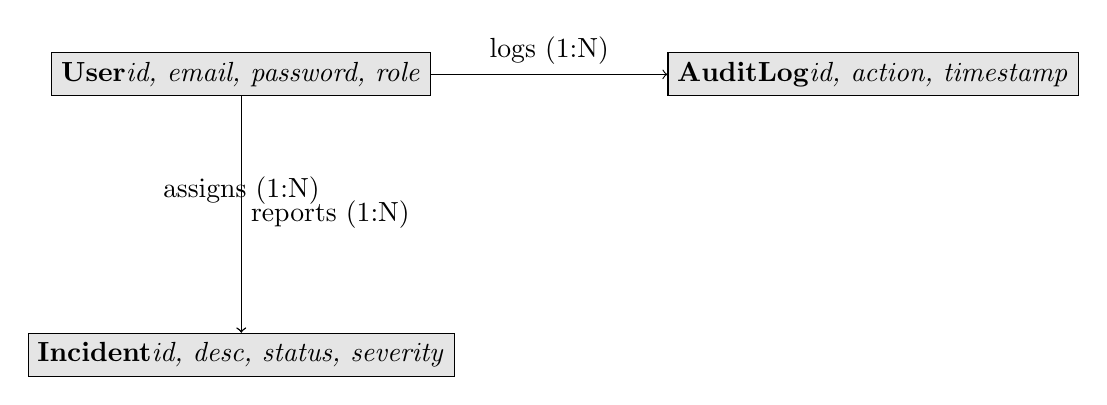
\begin{tikzpicture}[node distance=3cm]
        \node (User) [rectangle, draw, fill=gray!20] {\textbf{User} \\ \textit{id, email, password, role}};
        \node (Incident) [rectangle, draw, below=of User, fill=gray!20] {\textbf{Incident} \\ \textit{id, desc, status, severity}};
        \node (Logs) [rectangle, draw, right=of User, fill=gray!20] {\textbf{AuditLog} \\ \textit{id, action, timestamp}};
        
        \draw[->] (User) -- node[right] {reports (1:N)} (Incident);
        \draw[->] (User) -- node[above] {assigns (1:N)} (Incident);
        \draw[->] (User) -- node[above] {logs (1:N)} (Logs);
    \end{tikzpicture}
    \caption{Simplified ER Diagram (Derived from Models)}
    \label{fig:erd}
\end{figure}

\subsection{Table Specifications}
\begin{description}
    \item[User]: Stores credentials. Roles: `admin`, `officer`, `user`.
    \item[Incident]: The core entity. Includes `image_path` (file reference) and `ai_labels` (JSON).
    \item[MapNode]: Represents points on the campus graph for navigation (Graph structure).
\end{description}

\section{Frontend Design \& HCI}
The frontend uses Server-Side Rendering (SSR) with Jinja2.

\subsection{User Flows}
\begin{enumerate}
    \item \textbf{Login Page} (\texttt{login.html}): Simple email/password form.
    \item \textbf{Dashboard} (\texttt{dashboard.html}): Shows "Active", "Critical", and "Recent" stats cards.
    \item \textbf{Map View} (\texttt{map.html}): Interactive Leaflet.js map.
\end{enumerate}

\subsection{Usability Analysis}
\begin{itemize}
    \item \textbf{Accessibility}: Toast notifications are used for feedback rather than silent failures.
    \item \textbf{Responsiveness}: Dashboard uses Bootstrap `col-md-3` grid, ensuring it stacks on mobile.
    \item \textbf{Observation}: The login form might be small on high-DPI mobile screens (Needs CSS tweak).
\end{itemize}

\begin{figure}[h]
    \centering
    \begin{tikzpicture}
        \node[draw, minimum width=8cm, minimum height=5cm] {PLACEHOLDER - Screenshot of Dashboard};
    \end{tikzpicture}
    \caption{Web Dashboard Interface}
\end{figure}

\section{Security Analysis}
\begin{enumerate}
    \item \textbf{Authentication}: Hybrid approach implemented in `app/utils/jwt_auth.py`. Allows seamless transition between Web (Cookie) and API (Token).
    \item \textbf{CORS Configuration}: Currently set to `*` in `app/__init__.py`. \textbf{Recommendation}: Restrict to specific domains for production.
    \item \textbf{Sensitive Data}: Passwords are hashed using PBKDF2 (Werkzeug).
\end{enumerate}

\section{AI Integration Status}
\textbf{Status}: Mock / Stubbed. \\
The file `app/services/ai_analyzer.py` contains the structure for analysis but currently returns randomized mock data.

\begin{lstlisting}[language=Python, caption={Mock AI Logic}]
def analyze_image_mock(image_bytes):
    # TODO: Replace with HuggingFace API
    severities = ['LOW', 'MEDIUM', 'HIGH', 'CRITICAL']
    return {
        'severity': random.choice(severities),
        'confidence': round(random.uniform(0.7, 0.99), 2)
    }
\end{lstlisting}

\section{Deployment \& Run Instructions}
\subsection{Local Development}
\begin{lstlisting}[language=bash]
# 1. Install Dependencies
pip install -r requirements.txt

# 2. Initialize Database
python db_init.py
python seed.py

# 3. Run Server
python app.py
\end{lstlisting}

\subsection{Missing Implementation Action Items}
The following items were identified as missing during the audit:
\begin{itemize}
    \item \textbf{Real AI Model}: Needs connection to an inference API.
    \item \textbf{Email SMTP}: Forgot Password flow generates tokens but does not send emails.
    \item \textbf{Testing}: Unit tests exist for Auth but Maps logic coverage is low.
\end{itemize}

\section{Conclusion}
The CNSMS web application provides a robust foundation for campus safety. The hybrid authentication and modular architecture allow for easy scaling. Immediate next steps involve integrating the live AI model and securing the CORS policy for deployment.

\appendix
\section{Repository File List}
\lstinputlisting[language=Python, caption=repo-files.json]{repo-files.json}

\end{document}
